\documentclass[12pt,a4paper,openright]{article}
\usepackage[latin1]{inputenc}
\usepackage{amsmath}
\usepackage{amsfonts}
\usepackage{amssymb}
\usepackage{graphicx}
\author{Fabio Busignani}



\usepackage[usenames,dvipsnames]{xcolor}
\usepackage{tikz}
%%%<
\usepackage{verbatim}
%\usepackage[active,tightpage]{preview}
%\PreviewEnvironment{tikzpicture}
%\setlength\PreviewBorder{10pt}%
%%%>

\usetikzlibrary{arrows,shapes,positioning,shadows,trees}

\tikzset{
  basic/.style  = {draw, text width=2cm, drop shadow, font=\sffamily, rectangle},
  root/.style   = {basic, rounded corners=2pt, thin, align=center,
                   fill=MidnightBlue!80},
  level 2/.style = {basic, rounded corners=2pt, thin,align=center, fill=ForestGreen!30,
                   text width=8em,drop shadow,},
  level 3/.style = {basic, thin, align=center, fill=YellowGreen!15, text width=6.5em, rectangle}
}

\begin{document}
\begin{figure}
\centering
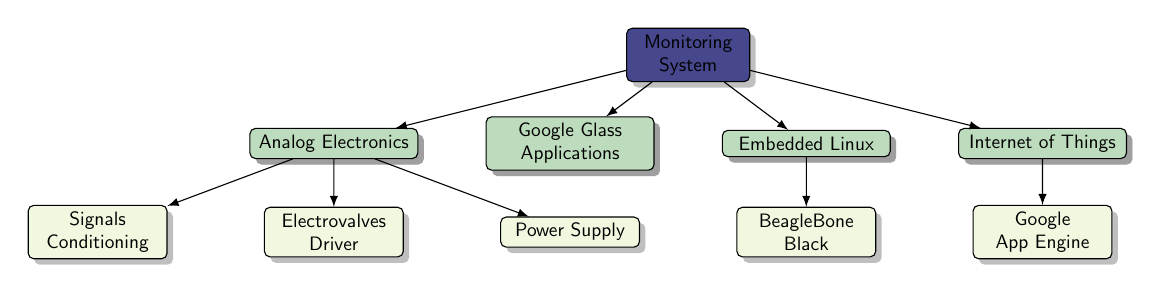
\begin{tikzpicture}[
  level 1/.style={sibling distance=40mm},
  edge from parent/.style={->,draw, black},
  >=latex, scale=0.75, every node/.style={scale=0.70}]

% root of the the initial tree, level 1
\node[root] {Monitoring System}
% The first level, as children of the initial tree
  child {node[level 2] (c1) {Analog Electronics}
  	child{node[level 3] {Signals Conditioning}}
  	child{node[level 3] {Electrovalves Driver}}
  	child{node[level 3] {Power Supply}}}
  child {node[level 2] (c2) {Google Glass Applications}}
  child {node[level 2] (c3) {Embedded Linux}
  	child{node[level 3] {BeagleBone Black}}}
  child {node[level 2] (c4) {Internet of Things}
  	child{node[level 3] {Google App Engine}}
  };
  





\end{tikzpicture}
\caption{Overview of the project}
\end{figure}
\end{document}